\documentclass{article}

% ———————————————————————————————————————————————————————
%  PACKAGES (1 seule fois chacun)
% ———————————————————————————————————————————————————————
\usepackage{geometry}
\geometry{a4paper,left=0.6cm,right=0.7cm,top=1cm,bottom=1cm,columnsep=0.8cm}

\usepackage{times}
\usepackage{paracol}
\usepackage{enumitem}
\usepackage{fontawesome}
\usepackage{tabularx}
\usepackage{tikz}
\usepackage{adjustbox}
\usepackage[hidelinks]{hyperref}
\usepackage{xcolor}
\usepackage{ragged2e}

\setlist[itemize]{itemsep=2pt,topsep=0pt,leftmargin=*}
\renewcommand{\labelitemi}{\textcolor{maincolor}{$\bullet$}}

\newcolumntype{Y}{>{\RaggedRight\arraybackslash}X}
\setlength{\parindent}{0pt}

% ———————————————————————————————————————————————————————
%  COULEURS & MISE EN PAGE
% ———————————————————————————————————————————————————————
\definecolor{maincolor}{HTML}{2AAEE7}
\definecolor{lightgray}{HTML}{A0A0A0}

% bande colorée à droite
\usepackage{eso-pic}
\AddToShipoutPictureBG{%
  \begin{tikzpicture}[remember picture,overlay]
    \fill[maincolor!10] (0.7\paperwidth,0) rectangle (\paperwidth,\paperheight);
  \end{tikzpicture}
}

% en-tête de section compact
\newcommand{\cvsection}[1]{%
  \par\bigskip
  {\Large\bfseries #1}\par
  \noindent\rule{\linewidth}{0.6pt}\par
  \medskip
}

% ———————————————————————————————————————————————————————
%  DOCUMENT
% ———————————————————————————————————————————————————————
\begin{document}\pagestyle{empty}
\columnratio{0.7}\begin{paracol}{2}

% ========== Colonne principale ====================================
{\LARGE\bfseries Judikael Mourouvin}

{\color{maincolor}\Large\bfseries Technicien informatique \& marketing digital}

\medskip
%----------- contact résumé ----------------------------------------
\begin{tabular}{@{}cp{0.45\linewidth}}
  \color{maincolor}\faEnvelope & \href{mailto:jkmou971@gmail.com}{jkmou971@gmail.com}\\
  \color{maincolor}\faPhone    &  {+590 0690 91 14 48}\\
  \color{maincolor}\faMapMarker& Route de Cocoyer\\ 97190 Gosier\\
  \color{maincolor}\faLinkedin & \href{}{}\\
\end{tabular}

\cvsection{PROFIL}
Passionné par l’informatique et le marketing digital, je combine une solide expertise technique en administration de systèmes et en support utilisateur. Mes expériences en mairie, chez Pôle Emploi et en PME m’ont permis de conduire des projets numériques variés et d’accompagner les équipes au quotidien. Rigoureux, pédagogue et orienté résultats, je souhaite désormais poursuivre à temps plein pour optimiser vos infrastructures et vos actions digitales. Disponible immédiatement, je m’engage à garantir la continuité et l’efficacité de vos services IT.

\cvsection{EXPÉRIENCE}

\colorbox{maincolor}{%
  \begin{minipage}{\linewidth}
    \textbf{Alternant en marketing digital} \\ Mairie du Gosier – DSI \\ 2023-2024
    \begin{itemize}
      \item Géré des projets numériques et coordonné leur déploiement auprès des services municipaux. \item Analysé les besoins des utilisateurs pour proposer des solutions adaptées et fiables. \item Assuré le support technique, formé les agents et contribué à la stratégie digitale de la collectivité.
    \end{itemize}
  \end{minipage}}

\vspace{3mm}


\colorbox{maincolor}{%
  \begin{minipage}{\linewidth}
    \textbf{Animateur de la zone informatique} \\ Pôle Emploi – Gosier \\ 2022-2023
    \begin{itemize}
      \item Assuré l’assistance et le support technique quotidien des conseillers et demandeurs d’emploi. \item Configuré, maintenu et sécurisé les postes de travail de l’agence. \item Diagnostiqué et résolu les incidents informatiques pour garantir la continuité de service.
    \end{itemize}
  \end{minipage}}

\vspace{3mm}


\colorbox{maincolor}{%
  \begin{minipage}{\linewidth}
    \textbf{Stagiaire informaticien} \\ Numerika – Baie-Mahault \\ 2020-2021
    \begin{itemize}
      \item Installé, configuré et dépanné divers équipements informatiques en atelier et chez les clients. \item Fournit un support utilisateur de premier niveau, améliorant la satisfaction clientèle.
    \end{itemize}
  \end{minipage}}   %← généré par build_placeholders()

\cvsection{FORMATION}

    \begin{tabularx}{\linewidth}{@{}c X@{}}
    \textcolor{sidetext}{\faGraduationCap} &
    \textbf{Bachelor Marketing Digital} \\
    & CFA IUTS \\
    & \begin{itemize}[leftmargin=*]
  \item Conception de stratégies de communication et gestion de campagnes en ligne. \item Analyse de données web et optimisation du référencement et des performances digitales.
\end{itemize} \\
    & \textit{2023-2024}
    \end{tabularx}
    

\vspace{3mm}


    \begin{tabularx}{\linewidth}{@{}c X@{}}
    \textcolor{sidetext}{\faGraduationCap} &
    \textbf{BTS Système Numérique option Informatique et Réseaux} \\
    & Lycée de Chevalier Saint-Georges, Abymes \\
    & \begin{itemize}[leftmargin=*]
  \item Étude des architectures réseau, protocoles et services d’infrastructure. \item Mise en œuvre de solutions de maintenance, d’exploitation et de sécurité des systèmes.
\end{itemize} \\
    & \textit{2019-2021}
    \end{tabularx}
    

% ———— Colonne de droite (bleue) ————————————————
\switchcolumn
\color{black}           % le fond est déjà maincolor!10

\centering
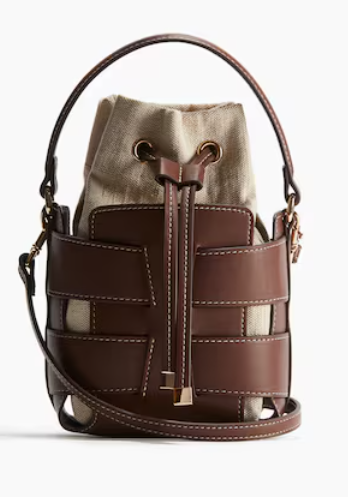
\includegraphics[width=3cm]{43f1eee0eba342f499d1a269b2735729.png}

\bigskip

\cvsection{COMPÉTENCES}

\begin{itemize}[leftmargin=*]
\item Support
\item Réseaux
\item Maintenance
\item Marketing
\item Configuration
\item Assistance
\item Diagnostic\end{itemize}


\cvsection{LANGUES}

\begin{itemize}[leftmargin=*]
\item English - \textcolor{gray}{}
\item Espagnol - \textcolor{gray}{}\end{itemize}


\cvsection{CENTRES D’INTÉRÊT}

\begin{itemize}[leftmargin=*]
\item Lecture \& veille technologique
\item Randonnée / sports outdoor
\item Voyages \& découverte culturelle
\end{itemize}


\end{paracol}
\end{document}
